
\begin{frame}
    \frametitle{Éco-résolution}
    \begin{block}{Principe de résolution}
  		 \begin{itemize}
   			 \item Ne raisonne pas de manière globale mais considère le problème comme des agents devant satisfaire un but
    			 \item Pas d'exploration globale de l'ensemble des états
    			 \item Une perturbation ne modifie que peu le mécanisme de résolution  
         \end{itemize} 
	\end{block}
	\pause
	\begin{alertblock}{Conclusion}
		Pour pouvoir appliquer l'éco-résolution il faut définir un ensemble d'agent dont le but est de tendre vers un état stable.
	\end{alertblock}
\end{frame}

\begin{frame}
    \frametitle{Éco-résolution}
    \begin{block}{Les éco-agents}
		 Ils sont caractérisés de la manière suivante :
  		 \begin{itemize}
   			 \item Un but : relation avec d'autres agents 
    			 \item Un état interne
    			 \item Fonction de perception de gêneur
    			 \item Volonte de satisfaire
    			 \item Obligation de fuir 
    			 \item Actions élementaires qui dépendent de l'application :
    			 faireSatisfaction(), trouverPlacePourFuir() et faireFuite()
         \end{itemize} 
	\end{block}
\end{frame}

\begin{frame}
    \frametitle{Éco-résolution}
    On peut voir l'éco-résolution comme un automate à états finis comme suit: 
    \begin{center}
        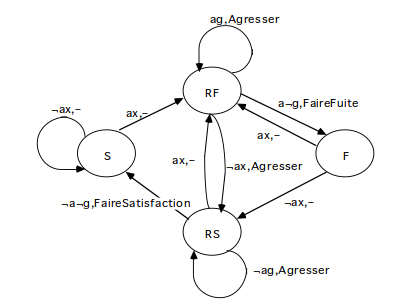
\includegraphics[scale=0.5]{images/AutomateEcoResolution.png}
    \end{center}
\end{frame}